\documentclass[10pt,a4paper,twocolumn,lineno]{article}
\usepackage[margin=.8in]{geometry}
\usepackage{graphicx}
\usepackage{amsmath}
\usepackage{amssymb}
\usepackage{titlesec}
\usepackage[numbers]{natbib}
\usepackage{sidecap, caption}

\titlespacing*{\section}
{0pt}{2ex}{0ex}
\titlespacing*{\subsection}
{0pt}{2ex}{0ex}
\titlespacing*{\subsubsection}
{0pt}{2ex}{0ex}

\font\myfont=cmr12 at 16pt
\title{\myfont The Wisdom and Manipulability of Threads}
\author{Robin Engelhardt$^1$, Jacob Stærk-Østergaard$^1$ and Vincent F. Hendricks$^1$ \\ 
		\textit{\small $^1$ Center for Information and Bubble Studies, Department of Communication,} \\ 
		\textit{\small University of Copenhagen, Karen Blixens Plads 8, DK-2300 Copenhagen S.}
		}
\date{}

\begin{document}
\twocolumn[
  \begin{@twocolumnfalse}
    \maketitle
    \begin{abstract}
\noindent
Social decision-making is increasingly relying on digitized aggregates of people’s opinions and judgments. These aggregates are frequently created and maintained as threads, i.e. as sequences of posts on a website. While it has been shown that knowledge of thread aggregates can distort individual decision-making, it is unknown how the ability to see preceding posts in a thread may influence collective accuracy, i.e. the wisdom of crowds. We therefore investigate experimentally the accuracy of threads in which people make numerosity estimations of varying difficulty and varying degrees of social information in the form of visible preceeding estimates. We find a significant increase in collective accuracy for high numerosities and high social information in non-manipulated threads, while in manipulated threads collective accuracy declines quickly under the same conditions. Our result suggests people tend to rely on social information more when tasks are more complex, and that pristine threads without manipulations indeed can improve collective decision-making. Using gaussian mixture models fitted by an expectaion-maximization (EM) algorithm we can gain additional insights into how people use the social information provided.
\\
    \end{abstract}
  \end{@twocolumnfalse}
]

\section{Introduction}
\noindent
Social information in the form of opinions and judgments by other people is sampled sequentially. We read the news, hear rumors, listen to debates on TV, and flip through comments on social media platforms and blogs. These activities inform us and influence our decisions, but researchers still debate the conditions under which these types of social information help us make better decisions \cite{woolley2010evidence, gurccay2015power, becker2017network, jayles2017social}, lead us astray \cite{caplan2011myth, lorenz2011social, minson2012cost, king2011true, le2018endogenous}, or just make us confused at a higher level \cite{salganik2006experimental, salganik2009web}. Collective estimates of a diverse group of people can outperform the majority of its members because any random confusion at the individual level is likely to average out and let the most accurate estimate prevail \cite{galton1907vox, muth1961rational, surowiecki2005wisdom, hong2008some}. Then again, confusion is not always randomly scattered around the truth. Systematic biases in individual perception may create measurable disruptions in the wisdom of crowds \cite{izard2008calibrating, nash2014curious, kao2018counteracting}. Social information can add to those biases and create cascades, echo chambers, bandwagoning and herd behavior \cite{anderson1997information, bikhchandani1992theory, bakshy2015exposure, banerjee1992simple}. Partially sampled social information may lead to rich-get-richer dynamics \cite{barabasi1999emergence} and to belief misattributions, which uphold harmful social practices despite being rejected by a majority of people \cite{katz1931students, darley1968bystander, ross1977false, noelle1974spiral, lee2019homophily}. Social information may also have been intentionally filtered or manipulated in various ways, for instance through group pressure \cite{asch1951effects}, algorithmic filtering \cite{pariser2011filter}, false cues \cite{salganik2006experimental, muchnik2013social, hanson1996hits}, or simply by plain misinformation \cite{hendricks2018reality}, often with highly detrimental consequences for our economy and our health.

%\noindent\fbox{%
%    \parbox{\linewidth}{%
%        \textbf{Significance} \\
%        Online discussion threads are important means for individual decision-making as well as for the aggregation of collective judgments, e.g the 'wisdom of crowds’. Empirical and theoretical investigations of the wisdom of crowds are currently ambivalent about the role played by social influence. While some findings suggest that social influence undermines crowd accuracy due to correlated judgment errors, others show that accuracy improves. We demonstrate that for difficult tasks, seeing previous estimates in a thread aids individual decision-making as well as the wisdom of crowds. However, when threads are artificially filtered in such a way that participants only see the highest estimates yet made, individual accuracy as well as thread accuracy declines dramatically.
%    }%
%}


Observational data of decision-making processes is acutely sensitive to the social context in which people find themselves. Thus, researchers find it difficult to separate observational data into its social and individual components. How may we know how much weight an individual puts on her own ‘independent’ estimate relative to the weight put on the estimates by others? Randomized experimental studies have attempted to solve this problem by first letting participants make a magnitude estimate of an object without social information, and subsequently ask them to revise their estimate after having received information about other people’s estimates of that object \cite{becker2017network, jayles2017social, lorenz2011social, sniezek1995cueing, mavrodiev2013quantifying}. This two-stage information paradigm presumes that people change their mind because of the social information they have received. Other studies, however, have shown that people routinely can change their mind all by themselves, and that it may be more correct to assume an `inner crowd' in the sense that people sample randomly from a probability distribution in their own mind \cite{vul2008measuring, herzog2009wisdom, herzog2014harnessing}. This may make it difficult to differentiate between `inner' samplings and `outer' influences, and it would be preferable to have methods that can infer directly the degrees of individual bias and social influence a single measurement. In real life people rarely estimate twice and rarely have access to all the relevant social information. So if we wish to make somewhat realistic experiments, we should create situations in which people see only a small fraction of the social information out there. In addition, the social information is rarely sampled at random. People typically collect social information from certain people, in certain places and in certain time intervals, for instance via a discussion thread, in user reviews, or in similar successive pronouncements after which they make up their mind. The effects of the clustered, sparse, and sequential nature of social information on decision-making have not been investigated systematically before and turn out to have a substantial impact on both individual decision-making and on the accuracy of the crowd. In particular, we will show that seeing preceding estimates in a thread improves collective accuracy when a) the task is difficult, b) the number of visible previous estimates is high, and c) the thread is pristine and unmanipulated in the sense that there is no filtering or rearrangement of preceding estimates. If, on the other hand, previous estimates are manipulated in such a way that people see only the highest (or lowest \footnote{Data not reported here}) estimates done so far, accuracy decreases dramatically. We will also show that it is possible to reliably infer the degrees of individual bias and social influence from a single estimate and its associated social information by using gaussian mixed models fitted by an expectaion-maximization (EM) algorithm. Such models give very good fits by allowing for a more complex mean/variance relationships, and provide insights into the highly variabe use of social information within each thread.
	

\section{Experimental Design}
We created a number of online threads, where a total of 10,348 participants could make magnitude estimations of varying difficulty and with a varying number of visible preceding estimates. Participants were asked to either estimate the number of dots in one of four images each showing a certain number of dots, or, honoring Francis Galton \cite{galton1907vox}, to estimate the weight of an ox on a photo together with information about the height and weight of a man standing next to it (see SI Appendix for screenshots of the experimental design). Dot estimation tasks have a long tradition in numerosity experiments \cite{minturn1951effect, indow1977scaling, krueger1982single} and have only recently been adopted as a useful ‘model organism’ for crowd aggregation research \cite{horton2010dot, ugander2015wisdom}. The true numbers to be estimated by the participants may be interpreted as varying ‘task complexity’, which in the following will be expressed by the categorical variable $d \in \{55$ dots, $148$ dots, $403$ dots , $1097$ dots, $1233$ kilo$\}$ (with an expected ordering for the dots-experiments, but not necessarily with respect to the ox-experiment), while the visible estimates by preceding participants in a thread, $v \in \{0,1,3,9\}$, may be interpreted as the degree of ‘social information’ available. Participants were placed randomly in one of the 20 thread configurations ($d \times v$ treatments) and made their estimate one after another. Treatments with $v=0$ thus correspond to a control condition for each $d$ that contain no social information. 

In order to test for the manipulability of threads, we ran $5 \times 3$ additional treatments with 4,522 participants that saw the same five images, but instead of seeing the $v$ preceding estimates, saw the $v$ \textit{highest} estimates made so far. This is a very heavy-handed type of thread filtering which we presumed would nudge participants to make ever higher estimates.\footnote{In order to keep the $v$ observed estimates in a somewhat realistic range, participants were not able to see estimates made that were above 100.000 and 10.000 in the  dots- and ox-experiments, respectively. See Materials and Methods for additional information about the handling of outliers.} No participant who had seen a certain image would be able to participate in another treatment containing the same image again. In addition to a participation fee and a variable waiting fee, all participants in all treatments received a bonus of \$1 if their estimate was within 10\% of the true value. See the Materials and Methods section and the Appendix for additional information about the experimental design.

\section{Methods}

\subsection{Aggregate Data}
\noindent
We model the log-error of thread medians, defined as $log_n(md_{(d,v)}/T)$, where $md_{(d,v)}$ are the thread medians and $T$ is the true value, as a function of $d$ using a generalized linear regression model...,

\subsection{Individual Threads}
\noindent
We use a mixture model to divide datapoints into states with corresponding independent gaussian components. Let $Y$ denote the observation and $X\in\{1,2,\dots,k\}$ denote the state. Then the conditional variable $Y|X$ is gaussian with parameters depending on the state $X$. 
As an example, let $X=\{1,2,3\}$, i.e. we assume a model with $k=3$ possible states. Then $Y|X=i \sim \mathcal{N}(\mu_i,\sigma_i^2)$ for $i=1,2,3$. Using notation $\delta = (\delta_1,\dots,\delta_k)$ as the estimated weight of each state, with $\delta_i >0$ and $\sum_{i=1}^k\delta_i = 1$, then the unconditional distribution of $Y$ becomes
$$
  P(Y) = \sum_{i=1}^k \delta_i P(Y|X=i),
$$

that is a weighted sum of gaussian probabilities, hence the name *gaussian mixture model* (GMM). This model structure can compensate for the heavy tails by adapting the different states to the more/less extreme observations. The number of states can be determined either by pre-specifying $k$ or use an information criteria such as AIC: $6k-2\log L$ or BIC: $3k\log(n)-2\log L$ (note that both criteria are scaled with $3k$ parameters for $k$ states), to pick a suitable number of states. Here BIC penalizes the number of parameters weighted by the ($\log$) number of states as $3k$, corresponding to $(\delta_i,\mu_i,\sigma^2_i)$ for each state, whereas AIC only penalizes by a factor 2. 

To keep things tractable we opt for a mix of specifying and using BIC where we set the number of states to $k\in\{2,3,4\}$ and then pick the number of states with the lowest BIC, conditional on convergence in the fitting routine. The model is fitted by the expectaion-maximization (EM) algorithm using the `depmixS4` package in `R`.

In order to account for other variables, the $\mu_i$ parameter can be extended, as in standard a linear regression model, with linear coefficients $\beta_{ij}, i=1,\dots,k, \quad j=1,\dots,p$. The specification of the mean $\mu_i$ is very flexible and can be adapted to each specific case. Here we opt for a model that can account for the social information present and in a special case a previous estimate for a given question, given prior to seeing social information.

\subsubsection{Specific model for data analysis}
\noindent
Given $N$ estimates $e_l, l=1,\dots,N$ from participants, we model the $\log$-error $y_l = \log e_l/T$, where $T$ denotes the true answer. Hence $y_l$ is comparable among different questions, but obviously the location and deviation depends on the difficulty of the question. Harder questions tend to exhibit more devation from the true value and $y_l$ tend to display a negative bias, often more pronounced when the true answer is of a high numerical value.

Each observation is associated with a piece of social information, i.e. previous estimates. In the setting of our experiments this amounts to a varying number of estimates: 0,1,3 or 9. In order to compare, we aggregate these into a single number $m_l$, namely the geometric average of the past $v$ observations: $m_l=\left(\prod_{s=1}^v e_{l-s} \right)^{1/v}$. Of course in the case of 0 observations, this variable is excluded as no information is available. In this case the model only report a bias value. We also analyze the dataset from Jayles, where a prior estimate $e_{l0}$ is given before any social information is revealed. Here we further include this estimate as explanatory. Hence we end up with 3 qualitatively different models for $\mu_i$, here we omit the state and observation depedent subscripts $i, l$ to ease readability

%$$
%\begin{align}
%  \mu &= \alpha & v=0\\
%  \mu &= \alpha+\beta_\text{social info}m & v>0\\
%  \mu &= \alpha+\beta_\text{social info}m +\beta_\text{prior}e_0 & \text{Jayles}\\
%\end{align}
%$$
Note that all of these models of the mean are state dependent.

\subsubsection{Model diagnostics}
\noindent
In order to evaluate a model fit, we calculate residuals. Here we exploit the fact that a sum of (independent) gaussian components is again a gaussian. Each observation $y_l$ has an associated weighting of each state. These weights are positive and sum to 1 and can thus be interpreted as probabilities. That is, given $k$ states, the model fits $k$ gaussians with mean and variance $\hat{\mu}_i, \hat{\sigma}_i^2, i=1,\dots, k$. For the $l$'th observation, we let $\hat{\delta}_{il}$ denote the assigned probability of this observation belonging to state $i$. Note that the number of states is fixed when fitting a model, hence it does not represent a true number, but merely an assigned number of states. However, given this particular number of states, the model optimizes the fit as of which state the given observation should belong to.
Hence, for each observation $y_l$, we can calculate the residuals first by substracting the weighted mean using $\hat{\delta}_{il}, i=1,\dots,k$. By scaling with the weighted variance analogously, we obtain centered and scaled residuals that should correspond to a standard normal $\mathcal{N}(0,1)$. So we obtain the following residuals (we use the subscript $l$ on the parameters to emphasize the possible dependency on expanatory variables associated with observation $l$)
$$
  \hat{\epsilon}_l = \frac{y_l-\sum_{i=1}^k\hat{\delta}_{il}\hat{\mu}_{il} }{\sum_{i=1}^k\hat{\delta}_{il} \hat{\sigma}_{il}}\sim\mathcal{N}(0,1)\quad l=1,\dots,N
$$

\section{Results}
In accordance with previous findings, participants do well when estimating small numbers independently. For higher numerosities, estimates vary widely and errors become substantial \cite{izard2008calibrating, krueger1982single, krueger1984perceived}. The median tends to underestimate the true value and the mean tends to overestimate the true value \cite{kao2018counteracting}. In comparison to Galton for instance, who found only a 0.8\% difference between the median estimate and the true weight of the slaughtered ox \cite{galton1907vox}, we find the median estimate to be less than half the true weight of the ox, as can be seen in the control condition $v=0$ in the top left panel of fig. \ref{fig:1}.

\begin{figure*}[!ht]
\centering
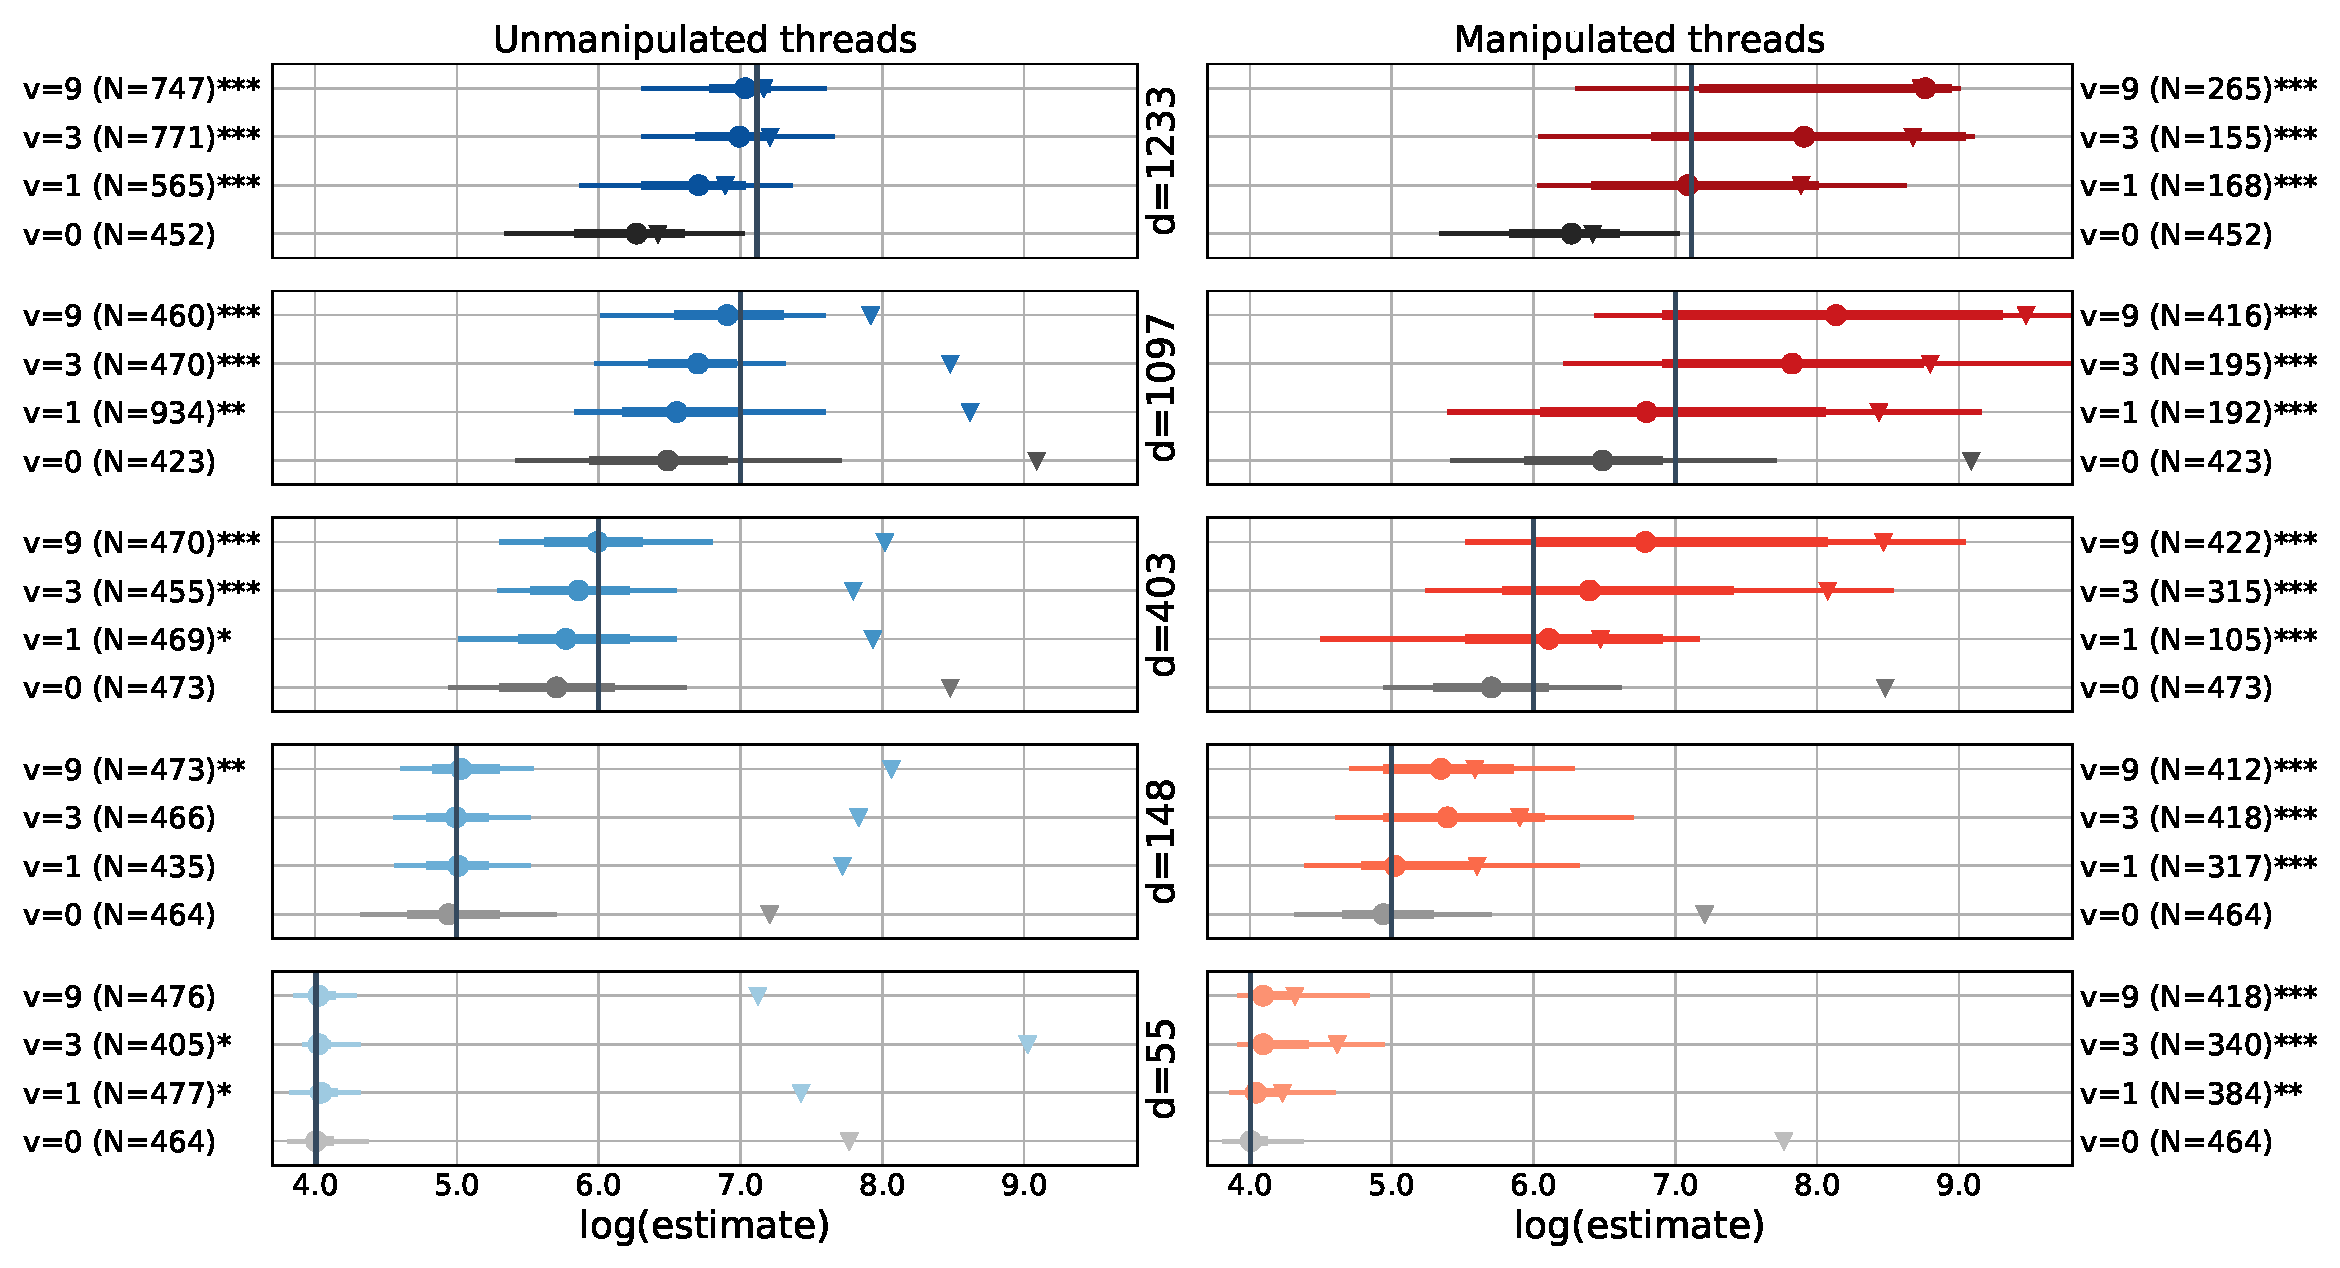
\includegraphics[width=1\linewidth]{../plots/fig1max.pdf}
\caption{\small \textbf{Left:} Summary statistics of $d \times v$ treatments with a total of 10.348 magnitude estimates of either the number of dots in an image, $d \in \{55,148,403,1097\}$, or the weight of an ox, $d \in \{1233\}$, while participants are able to see $v \in \{0,1,3,9\}$ preceding estimates. Greys are the control treatments with $v=0$. Estimates are log-transformed. Large circles indicate medians, triangles indicate arithmetic means, thick lines show interquartile ranges, thin lines show interdecile ranges, vertical black lines show the true value, and stars indicate significance levels compared to the control treatment (two-sided Wilcoxon-Mann-Whitney test). No outliers were removed, making the arithmetic means strongly right skewed. \textbf{Right:} Summary statistics of $d \times v$ treatments with a total of 4.522 additional magnitude estimates, where participants do not see the preceding estimates but the $v \in \{1,3,9\}$ \textit{highest} estimates made so far. The controls, $v=0$, are the same as on the left hand side.}\label{fig:1}
\end{figure*}

\subsection{Unmanipulated threads}
As soon as participants can see preceding estimates, accuracy improves substantially in difficult tasks, see the horizontal boxplots on the left hand side of figure \ref{fig:1}. Increasing the view count $v$ does not significantly improve collective accuracy in images with 55 and 148 dots. But as soon as the number of dots increases, social information starts to improve accuracy. And the larger the view count $v$, the more accurate the median (circles) becomes. Arithmetic means (triangles) quickly tend to overestimate the true value because free response elicitation of absolute values creates right-skewed, approximately log-normal distributions with a long tail, which inflate the means.\footnote{Due to the outliers, means become highly uninformative. Even when defining a cut-off for outliers, such as an error rate of 10, would still make the arithmetic means right skewed. Galton disliked the use of the mean for this very reason as it “would give a voting power to ‘cranks’ in proportion to their crankiness” \cite{galton1907vox}. While it is still debated \cite{kao2018counteracting} which measure is best suited to aggregate social information, we focus on the median: The median is easy to interpret, is robust against outliers, and best expresses the opinion of the crowd since the majority of participants in the thread deems every other estimate as too high or too low. See also the Appendix for a discussion of outliers.} The interquartile and interdecile ranges show how high difficulty, $d$, leads to higher diversity (i.e. variation) in the dots-experiments, while a higher view-count tends to reduce variation when $d$ is fixed, although not always.

\subsection{Manipulated threads}
The right hand side of figure \ref{fig:1} shows the equivalent results for manipulated threads. While participants are relatively unaffected by social information when difficulty is low in the unmanipulated threads, participants in the manipulated threads quick start to overestimate, even with $v=1$. For higher $d$'s and $v$'s, estimates inflate ever more. In fact, we were able to create threads in which a majority of participants estimated the ox ($d=1233$) to weigth more than 6000 kilo. Clearly, in the begining of a thread, only a few of the observed estimates are high numbers, making it not so probable for new participants to get influenced by them. But when threads become longer, still more of the observed estimates are very high numbers, making it more difficult to resist their influence. At a certain point, all visible estimates may be so improbably high, that participants may suspect foul play and start to ignore them. In some threads this effect can be observed by estimates branching off into two directions: those estimates showing herd behaviour by following the extremely high estimates seen, and those estimates ignoring them, see appendix figs 6 \& 7 for examples. This may contribute to the high variance of the manipulated threads. Also note that for $v=1$, the medians of the manipulated threads are often much closer to the true value than it is the case in the corresponding controls. This is so because the size of the manipulation (in this case showing only the single highest estimate in the thread) is just about enough to compensate for the naturally occuring underestimations in the controls.

\begin{SCfigure*}[][t]
\caption[Collective and individual performances]{\small
Collective and individual performances across $d$ and $v$. In unmanipulated threads (blues), collective and individual errors decrease. In manipulated threads (reds), errors increase. \textbf{a}: In unmanipulated threads, the collective error, $RE_C$ - i.e. the error of the median ($|truth-median|/truth$), drops substantially for high $d$ and with higher $v$. Confidence intervals (95\%) are show in error bars. \textbf{b}: In manipulated threads, collective errors increase dramatically for higher $d$ and $v>1$. The large error bar for $v=3$ indicates that a large minority makes very high estimates. \textbf{c}: In unmanipulated threads, the median individual error, $MdRE$ - i.e. the median of $RE = |truth-estimates|/truth$, drops substantially for higher $d$ and $v$, while for low $d$ it is small and independent of $v$. \textbf{d}: In manipulated threads, the median individual error increases strongly for high $d$ and high $v$, while again being independent of $v$ when $d$ is low. \textbf{e}: The WOC-index, W, measured as the fraction of participants who are worse than the error of the crowd median, $RE_C$, increases in general for higher $v$ in unmanipulated threads, demonstrating an increasing wisdom of crowds-effect. \textbf{f}: In manipulated threads, the crowd becomes less wise, except for $v=1$, which is due to the cancelling out of two opposing forces: a general underestimation bias and the influence of one observed high estimate.  $N$ shows the total number of estimates. No outliers were removed.
}
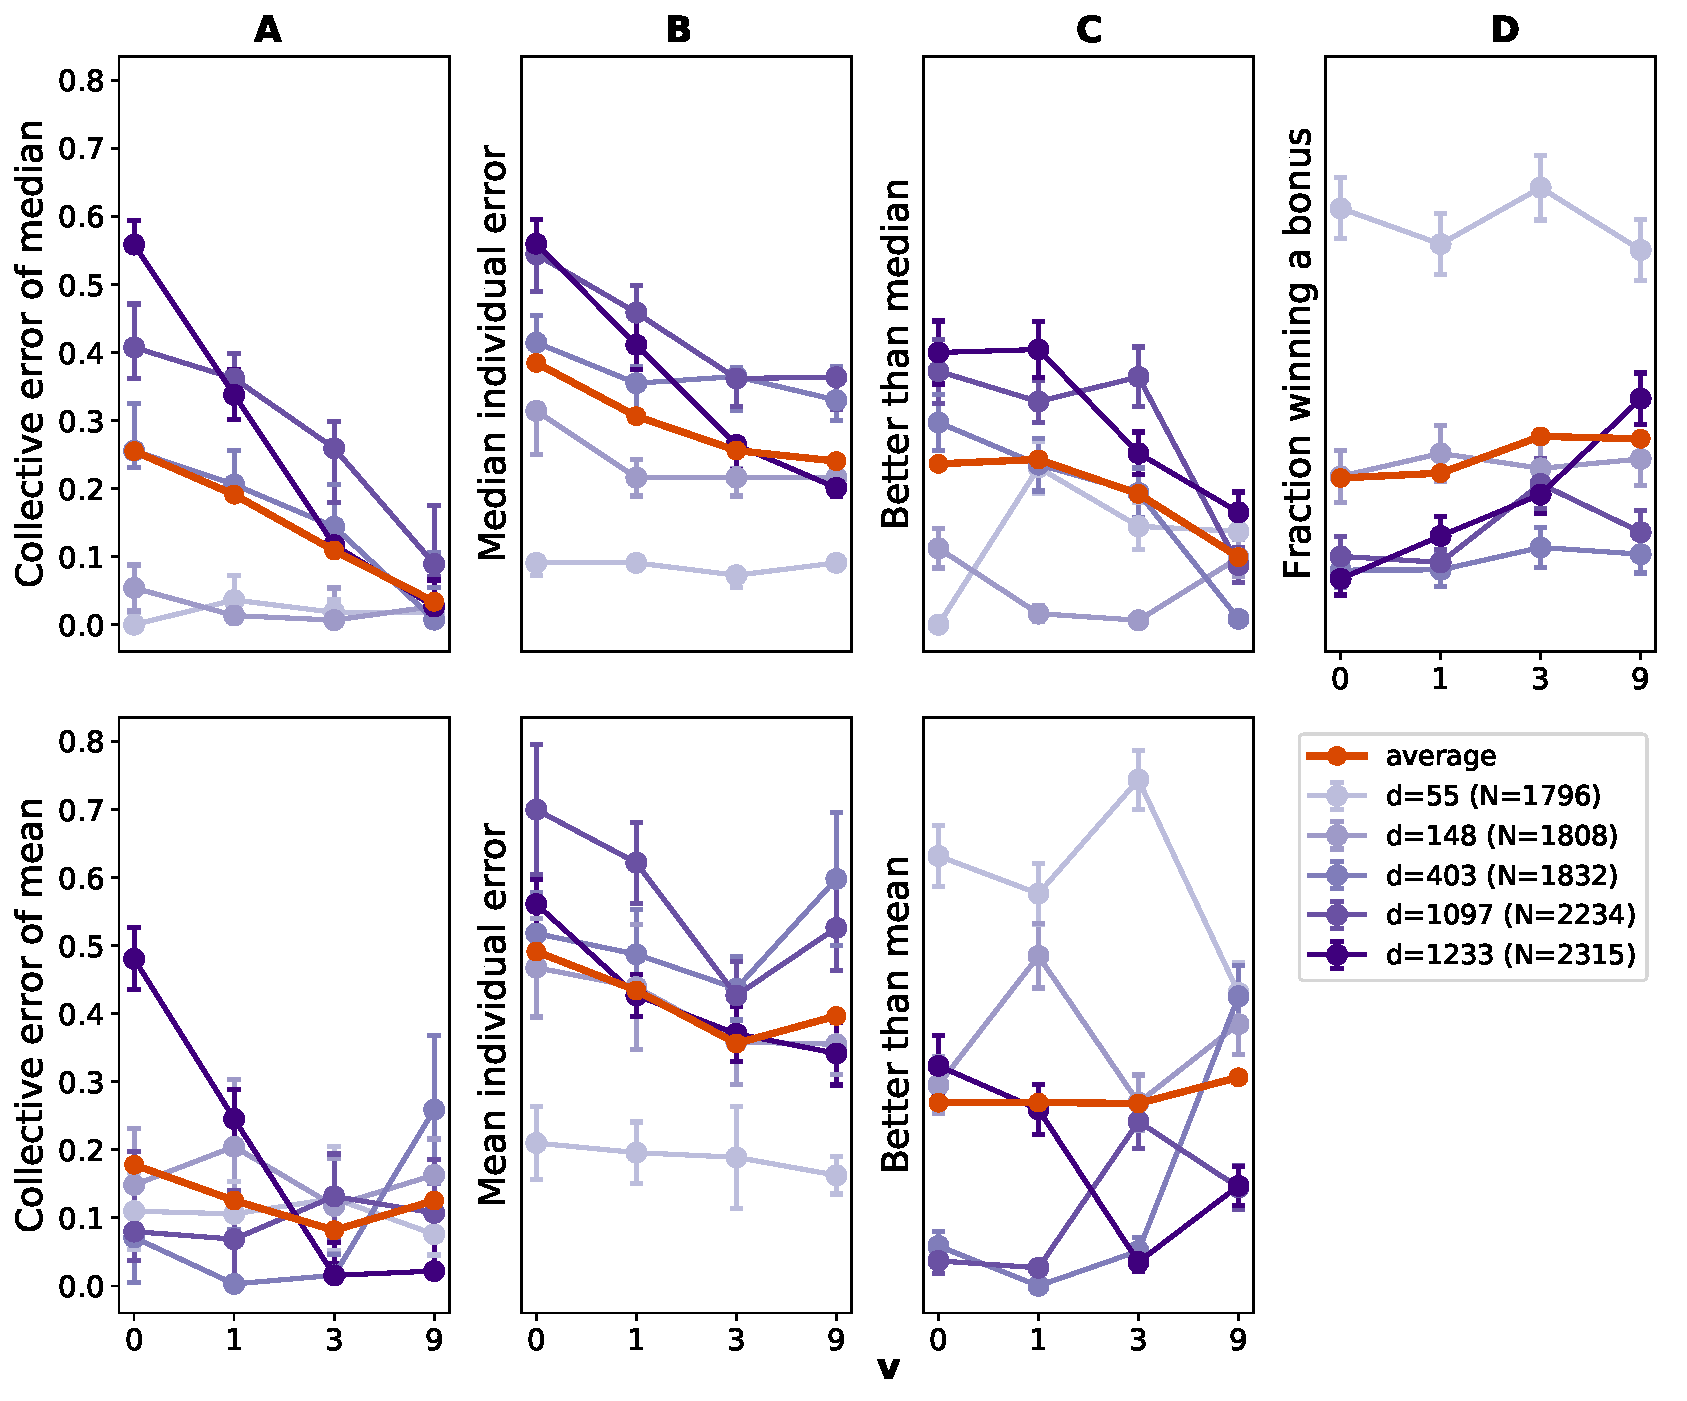
\includegraphics[width=.5\textwidth]{../plots/fig2.pdf}
\label{fig:2}
\end{SCfigure*}

\subsection{Collective and individual performance}
Figure \ref{fig:2} shows the benefits of social information for collective estimation accuracy (subplot \textbf{a}) and for individual estimation accuracy (subplot \textbf{c}) in unmanipulated threads. The effect is strong and robust in complex tasks with $d=\{403, 1097, 1233\}$. When threads are manipulated, however, the same reliance on social information creates very inaccurate collective as well as individual estimates (subplots \textbf{b} and \textbf{d}). For example: While the collective error of the median in the control with $d=1097$ is 0.4, the error decreases to 0.1 when participants can see nine preceding estimates ($v=9$), witnessing a highly beneficial effect on collective performance. Thus, a main result of the experiments is that participants tend to rely on social information more when the task is more complex, and that this reliance aids their decision-making as well as the wisdom of crowds in unmanipulated threads. The same reliance, however, leads to a very high collective and median individual error in complex tasks when the \textit{highest} estimates are shown. While participants are able to calibrate their own estimation towards a more accurate value when they see preceding guesses, they are led astray as soon as these estimates have been purposefully changed. In a truthful world credulity is fine and well, but in a fraudulent one it is fatal.

A simple wisdom-of-crowds measure, $W$, is the fraction of participants who are less accurate than the median of the thread, i.e. 

$$
W=\frac{1}{N} \sum_i^N x_i, \text{ } x_i=
\begin{cases}
  1 & \text{if } RE_i > RE_C \\    
  0 & \text{otherwise }
\end{cases}
$$

\noindent
where $RE_i = |e_i-T|/T$ is the error rate of estimate $e_i$ by participant $i$, $RE_C = |md-T|/T$ is the error rate of the thread median, $T$ is the true value, and $N$ is the number of estimates. Figure \ref{fig:2}\textbf{e} shows that $W$ increases with increasing social information in the majority of cases, which means that less and less participants are better than the crowd median. Thus, increasing social information magnifies the wisdom of crowds effect in complex tasks. In contrast to \cite{lorenz2011social} and in concert with \cite{becker2017network, farrell2011social} this supports the claim that crowds indeed may become wise under social influence, even though wiser individuals give the aggregate wisdom of crowds measure a tougher baseline to compete against. 

In manipulated threads the WOC-index decreases as expected (figure \ref{fig:2}\textbf{f}), but is surprisingly high when participants see only the highest estimate in their thread at $v=1$. This resonates well with the findings in \cite{jayles2017social}, who showed that providing a moderate amount of incorrect information can counterbalance underestimation bias and improve collective performance. It is striking, however, that this manipulation works equally well in all threads (except in the easiest dot-experiment with $d=55$), and confirms that human numerosity underestimation bias indeed is systematic, predictable and `repairable' \cite{jayles2017social, kao2018counteracting, indow1977scaling, nash2017sequential}.
 
\subsection{Herd behavior}
\noindent
Visual inspection of thread dynamics (see minimal spanning trees in the Appendix, figs. S4-S7) reveals that most threads contain multiple occasions of herd behavior in the sense that participants frequently copy one of their preceding estimates. Prolonged herd behavior is rare in the unmanipulated dots-experiments (typically 1-5 instances in a thread of length 4-500), but common in the ox-experiments. Herd behavior drastically changes the visual appearance of the tree-like structure of the threads (see figures in appendix): Unmanipulated dot-threads typically show themselves as plump and well-formed trees with bushy branches, while ox-threads exhibit much sparser and fastigate (i.e. vertically aligned) branches, indicating that herd behavior is much more pronounced when people estimate the weight of an ox.


\begin{SCfigure*}[][t]
\caption[Herd behavior across tasks complexities and view counts.]{\small
Herd behavior across tasks complexities and view counts. (\textbf{a, b}): The probability difference between proportions, $\Delta_v = I(v) - I_0(v)$, is a simple measure of herd behavior under social influence. In unmanipulated threads (\textbf{a}), only the ox-experiment sees a continuous increase in herd behavior across all $v$, while most dot-threads have a peak at $v=3$. In the manipulated threads (\textbf{b}), $\Delta_v$ becomes negative in many threads, indicating that many participants do not belief the estimates they can see. Wald two-sided confidence intervals (95\%) are given in error bars. (\textbf{c, d}): The ratio of the proportions, $\Theta_v = \frac{I(v)}{I_0(v)}$, is in the majority of cases higher than unity, and significantly so in most ox-experiments (darkest blue and darkest red), and in most threads with $v=3$. As confindence intervals (95\%) we use the recommended \cite{fagerland2015recommended} Koopman asymptotic score interval as given by Nam \cite{nam1995confidence}. \textbf{e,f}:  The ratio of proportions of bonuses given when being an imitator and being not an imitator........ Color codings and sample sizes are the same as in figure \ref{fig:2}.
}
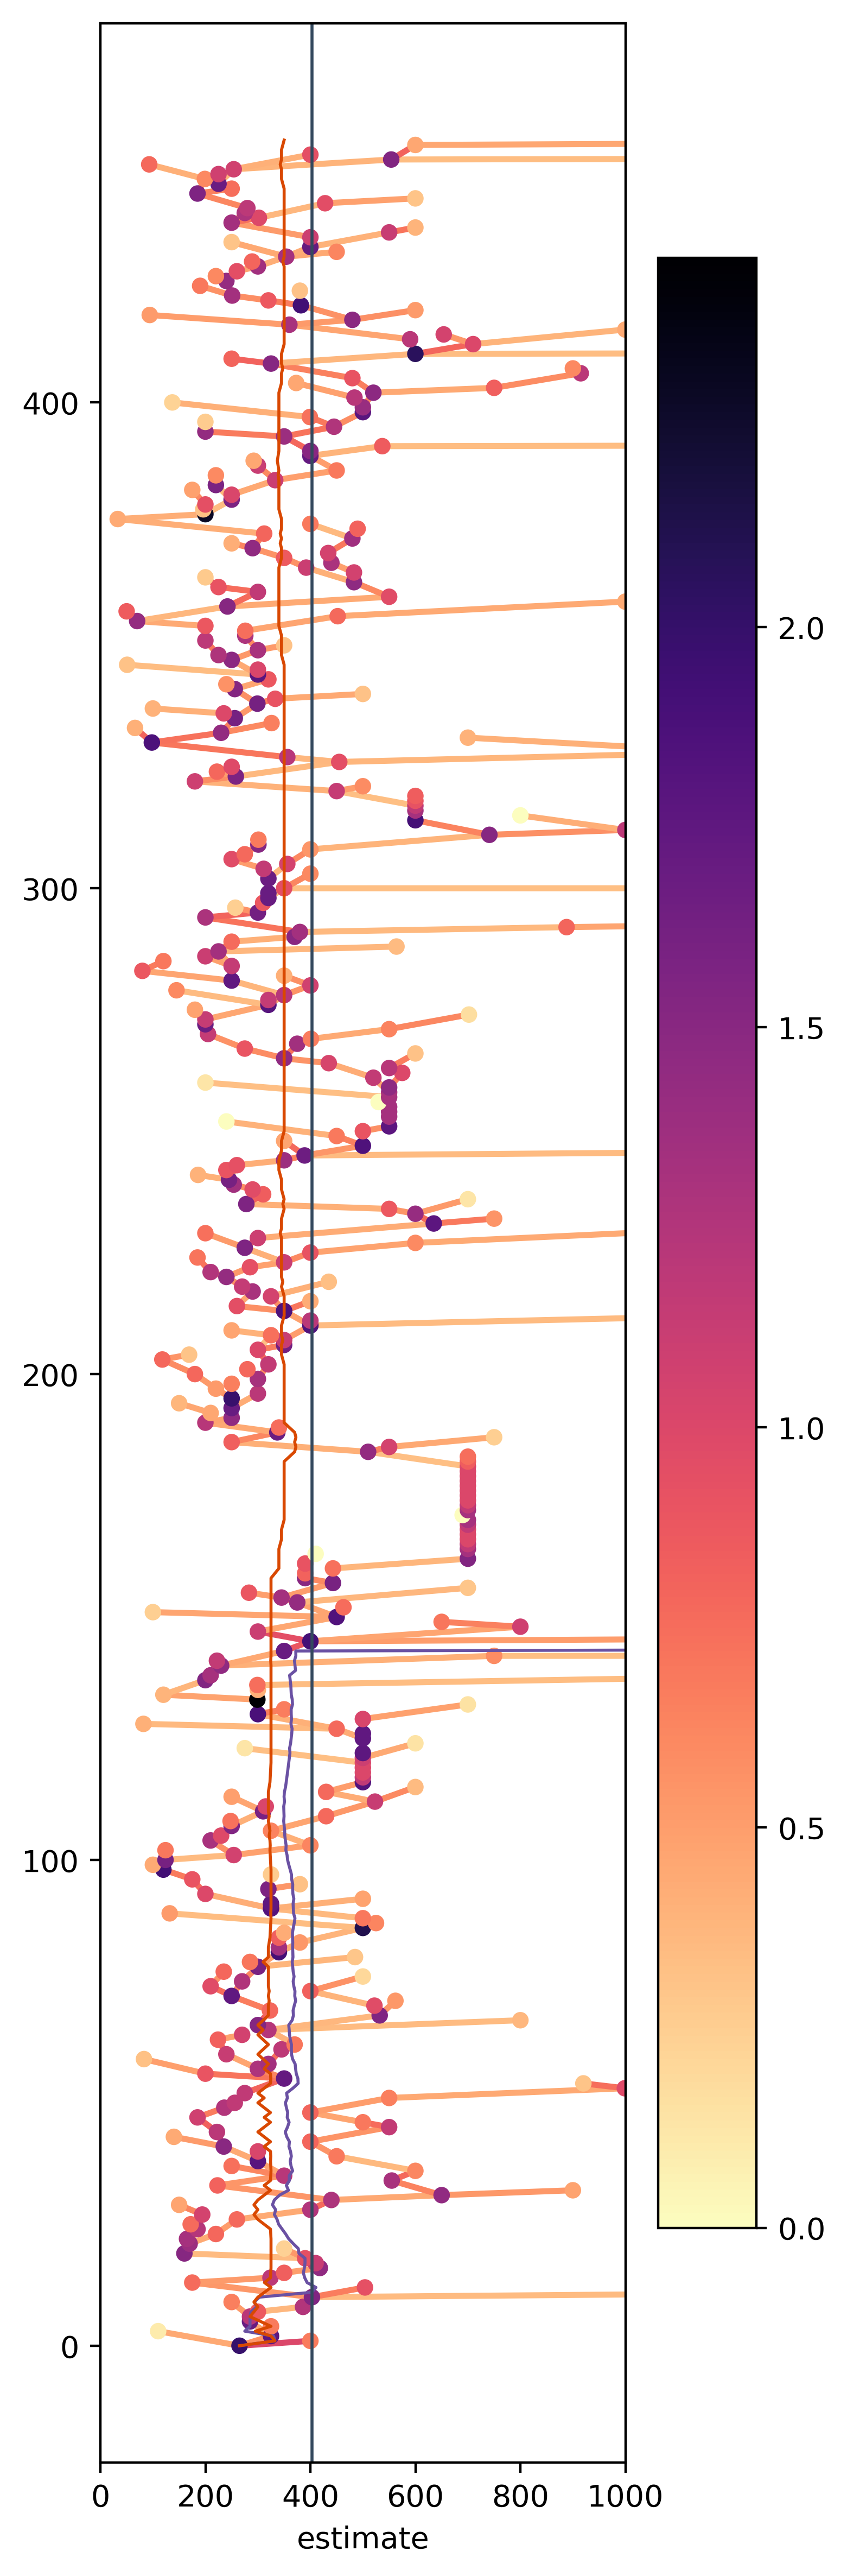
\includegraphics[width=.45\textwidth]{../plots/fig3.png}
\label{fig:3}
\end{SCfigure*}

As a simple point estimate of herd behavior we can use the proportion of participants who copy one of the preceding estimates they can see:

$$
I(v)=\frac{1}{(N-v)} \sum_{i=v}^N  x_i \text{, } x_i=
\begin{cases}
  1 & \text{if } e_i \in \{e_{i-1},..,e_{i-v}\} \\    
  0 & \text{otherwise }
\end{cases}
$$

\noindent
where $v$ is the number of visible estimates, and $N$ is the total number of estimates in a thread. Of course, some people may become copycats only by accident, for instance due to the limited number of good guesses available in less complex tasks, or due to mental rounding, focal points \cite{schelling1980strategy}, or simply by chance. The above proportion is therefore only informative when we compare it to the naturally occuring proportion of imitators in threads without social information, $I_0(v)$, which we estimate by counting how many times an estimate has occured by chance in $v$ preceding steps in the control experiments with $v=0$ (see table A1 in the appendix). 

The relationship between the two proportions $I(v)$ and $I_0(v)$ is shown in figure \ref{fig:3}a-d. Figures \ref{fig:3}a and b show their difference,  $\Delta_v = I(v) - I_0(v)$, giving an estimate of the overall magnitude of imitative behavior when social information is present. In contrast, figures \ref{fig:3}c and d show the ratio between the two proportions $\Theta_v = \frac{I(v)}{I_0(v)}$, which estimates how much more (or less) people tend to copy each other when they have social information compared to when they have no such information. So if $\Theta_v \approx 1$ (i.e.  $\Delta_v \approx 0$), the probability of imitation is no different from what would happen by chance. If  $\Theta_v >1$, imitation is on average $\Theta_v$ times higher than what would occur by chance, and if $\Theta_v <1$, imitation is less than what would occur by chance, which means that people look at preceding estimates mostly in disbelief.

Figures \ref{fig:3}a-d reveal that a majority of the complex unmanipulated threads have a positive probability difference ($\Delta_v >0$, $\Theta_v>1$), demonstrating that participants rely on social information more when the task is more complex. This relationship, however, is nontrivial: First, herd behavior is consistently higher in the ox-experiments (dark blues and reds) than in the dots-experiments ($p<0.05$ in 5 out of 6 ox-threads, but only in 10 out of 24 dots-experiments). Second, the willingness to copy previous estimates is much higher than chance when $v=3$ ($\mathit{p}<.05$ in 8 out of 10 threads) rather than when $v=1$ ($\mathit{p}<.05$ in 3/10) or $v=9$ ($\mathit{p}<.05$ in 4/10), which suggests that there may exist an optimal level of social information at which influence is maximized. Third, disbelief is not uncommon in low-complexity tasks, especially in the manipulated threads. This makes intuitively sense, because participants often see a bunch of highly inflated estimates in the manipulated threads, which may prompt them to make up their own mind instead.

Since the imitation proportions count only those people who make an exact copy of a predecessor estimate, we complement the analysis in the appendix with a more encompasing approach and include participants who make an estimate that is `close' to one or more predecessor estimates. Figure SXX in the appendix shows the cumulative distribution of such copycats in terms of their percentual distance, $p$, to one or more preceding estimates in unmanipulated threads with the highest complexity and the highest amount of social information. The extend of herd behavior beyond simple copying is again much more pronounced in the ox-threads, indicating that people use different strategies when estimating different things. 

---

blablabla..



%
%It turns out that herd behavior may be beneficial in the most complex tasks: the closer an estimate is to an estimate seen, the higher is the probability to win the bonus. As shown in Fig. \ref{fig:5}\textit{b}, all average relative win rates up to $p=10\%$ are higher than unity in the most complex tasks ($d=1097$ and $d=1233$), demonstrating that participants may increase their win rate when emulating each other. 
%
%Several threads also show signs of a bandwagon effect. Bandwagoning occurs when the rate of herd behavior increases with the number of copycats seen. We can construct a simple measure of herd behavior and associated bandwagoning by a `fastigation index', $F$, which calculates the average number of preceding estimates copied by each person in the thread:
%
%$$
%F(v)=\frac{1}{N-v} \sum_{i=v}^N \sum_{k=1}^v x_{i,k}, \text{ } x_{i,k}=
%\begin{cases}
%  1 & \text{if } e_i = e_{i-k} \\    
%  0 & \text{otherwise }
%\end{cases}
%$$
%
%where $e_i$ is the estimate by participant $i$, and $v$ is the view count so that $F \in [0,v]$. A fastigation index of zero would indicate no copying at all, and $F=v$ would indicate that all participants copy their previous estimate(s). Threads with $v=1$ will have a fastigation index equal to their imitation ratio, so while the imitation ratio measures the extend of herding, the difference between the fastigation index and the imitation ratio measures the extend of bandwagoning in a thread. Table \ref{table:1} summarizes the amount of bandwagoning in the most complex threads with 3 or 9 views. While bandwagoning in general is higher in manipulated threads, what stands out is the much ... An exception is the unmanipulated thread with $d=403$ and $v=3$ which had frequent episodes of long bandwagons, see figure XX in the appendix. 
%
%
%\begin{table}[h!]
%\centering
%\caption[caption]{% this is a trick in order to make some room under the caption text
%\small
%Bandwagoning, $B=F-I$, for threads with $d\in \{403,1097,1233\}$ and $v \in \{3,9\}$. $B_u$ and $B_m$ are the bandwagon effects for unmanipulated and manipulated threads, respectively. Robin remember to make significance tests here.\\\hspace{\textwidth}
%}\label{table:1}
%\begin{tabular}{rrrr}
%\hline
%    d &   v &      $B_u$ &       $B_m$ \\
%\hline
%  403 &   3 & 0.114   & 0.01 \\
%        &   9 & 0.016   & 0.111   \\
% 1097 &   3 & 0.011  & 0.129   \\
%         &   9 & 0.018  & 0.201   \\
% 1233 &   3 & 0.045  & 0.081  \\
%         &   9 & 0.211    & 0.294   \\
%\hline
%\end{tabular}
%\end{table}
%
%
%

\section{Discussion}
In the original wisdom of crowds experiment by Francis Galton, people estimated the weight of a “fat” slaughtered ox \cite{galton1907vox}. A multitude of formal and informal studies have subsequently tried to replicate Galton’s findings by using various other items, from coins and jelly beans to stock prizes and best movie nominations. This has happened even though researchers were quick to point out that the social context of such experiments, the attributes of the items such as their numerical magnitude \cite{izard2008calibrating, krueger1982single}, their extremeness and complexity \cite{nash2014curious, taleb2009errors}, as well as the expertise of the participants \cite{perry1907ballot}, are important factors to consider. 

The differences in the results of our dot-experiments and our experiment with an even stouter ox show that item attributes indeed matter. Estimating dots on a screen may or may not require as much expertise as estimating the stoutness of cattle, but the observed differences in the levels of herd behavior at least indicate that participants use different strategies when estimating different things. What does not differ, however, is a systematic underestimation bias of large numbers and a rapid improvement in individual as well as in collective accuracy when the number of visible preceding estimates is increased. 

This means that the social information contained in a thread in fact helps people to calibrate their own decision-making process, even if the information may be wrong. Concerns about gullibility and correlation of judgment errors may thus be less of an evil compared to the positive effects of seeing honest opinions from other people in a thread.

One possible reason for frequent herd behavior in the ox-threads is that participants are much more uncertain about their ability to estimate cattle weight compared to their ability to estimate dots on a screen. A high degree of uncertainty - or even an acceptance of cluelessness - may prompt participants to copy previous estimates rather than to make independent estimates by themselves \cite{navajas2018diversity}. 

%Our work also gives credence to some of the conclusions drawn by social learning models, which show that groups of naïve agents can become wise under certain conditions such as high dispersion of social information \cite{golub2010naive} and decentralized communication networks \cite{becker2017network}. It remains to be seen, however, how collective and individual accuracy performs in more realistic settings. Many existing online discussion threads attach additional social information to posted comments, such as counters of ‘likes’ and sub-threaded conversations. Others carry tags of seniority or expertise, and still other threads are ranked, filtered, or manipulated in various ways. Such alterations to the basic cascade structure of a thread significantly change the topology of the communication network and has largely unknown consequences for the individual decision-making process as well as for the collective performance. These are potential directions for future work.
%
%
%
%Since individual accuracy improves with increasing samples of social information in unmanipulated complex tasks, the relative accuracy of estimates compared to sample means must improve as well (SI Appendix, Fig. S4). It is not clear, however, how individuals are able to put more weight on those estimates that are closer to the true value than on estimates that are further away. 
%
%
%
%When inspecting the minimum spanning tree in Fig. \ref{fig:3}, it is clear that such branching points (the forks in the tree) are more centralized in comparison to the outer estimates. This suggests that the greater accuracy of high-influencers may be due to central limit effects of participants averaging the estimates they can see (their sample), rather than to an ability to endorse estimates that are more accurate. We test this hypothesis by simulating a ‘naïve social learning’ model of participants’ decision-making process, assuming that participants aggregate social and personal information evenly \cite{degroot1974reaching, golub2010naive}. Simulating such a model (see the Materials and Models section and the SI Appendix) shows that medians indeed converge towards the means for increasing $v$ (Fig. S8), indicating that at least a partial reason for the wiser threads is due to central limit effects of participants choosing an intermediate estimate. But the simulations also show no significant differences in error between high- and low-influencers (Fig. S9). This demonstrates that individual sample aggregation does not explain the increasing arithmetic means in the experiments, nor does it explain the large differences in accuracy between high- and low-influencers found in Fig. \ref{fig:4}. We may therefore conclude that participants in a thread indeed are able to find and to follow estimates that are more accurate. The second main result of this article is thus that in addition to a wisdom of crowds effect, high individual estimation accuracy translates into higher social influence among succeeding participants in a thread, and that this effect may compound in time, improving individual as well as thread accuracy even further (see SI Appendix and Fig. S10).
%
%It is ironic that our crowds are most wise only when they are manipulated properly. It remains to be seen...
%
%

\subsection*{Experimental design and data collection} Controlled experiments of thread dynamics are rare in the research literature due to the difficulties in keeping a large number of participants in a queue. We designed our experiment along the same lines as the classical information cascade experiments by Anderson and Holt \cite{anderson1997information}. While such a design is not very feasible in normal laboratory conditions (at least for threads with several hundred participants), it is well suited for online labor markets and crowdsourcing platforms such as Amazon Mechanical Turk (AMT, see SI Appendix for further discussions of the pro and cons of AMT). We thus recruited participants from AMT to make a total of 10.808 magnitude estimations in various threads containing either an image of a certain number of dots ($d \in \{55,148,403,1097\}$) or an image of an ox ($d=1233$). After accepting our ‘HIT’ (‘human intelligence task’) and providing informed consent, participants waited in a ‘waiting room’ until the ‘choice room’ became available. When entering the choice room participants could see an image d together with $v \in \{0,1,3,9\}$ estimates made by previous participants. After making an estimate, participants were thanked and paid a participation fee of \$0.10 and bonus of \$1 if their estimate was within 10\% of the true number. The average time used was less than two minutes, see SI Appendix for screenshots and more detailed descriptions of the design and setup.
%\subsection*{Outliers} We did set the minimum and maximum values submittable to be 10 and 1 million respectively. We however knew that our experiments still would be vulnerable to the dangers of free-response elicitation: 127 participants had an error rate above 10, and out of those, 62 participants had an error rate above 100. We therefore chose to trim our data when reporting aggregates. Using Tukey’s 1.5 IQR rule \cite{tukey1977exploratory} would be too exclusive however, because our distributions are not normal and because it has been previously reported that participants frequently make estimates with an error rate of 4 or more \cite{izard2008calibrating, kao2018counteracting, indow1977scaling}. The upper bound is therefore chosen to be any estimate above an error rate of 10, so that $|x_r-truth|/truth <10$, where $x_r$ is the estimate by participant $r$. We also use a lower bound of $truth/10$, due some initial reports of early timeouts and not being able to see the form input on mobile devices (see SI Appendix, section “AMT Settings”). In total, these bounds remove 254 (2.4 \%) estimates from the reported aggregate data. 
%\subsection*{Simulation model} An important question is to understand how social learning may contribute to the wisdom of threads. In order to do so, we model the individual decision-making process in such a way that all participants calculate the average of all estimates seen including their own ‘hunch’, $e_r$, of what the correct number might be. By denoting an individual’s estimate $x_r$ with $r \in N$ individuals in a thread, we can calculate subsequent estimates according to $x_r = \frac{1}{v+1} \big(e_r + \sum_{i=1}^{v} x_{r-i}\big)$, where $e_r$ is a tentative guess (‘hunch’) without social information, $x_{r-i}$ are the estimates seen and $v$ is the view count. Simulating this model with values from the control experiment as the initial hunches and with increasing degrees of social information, $v$, shows that the median indeed will shift towards the arithmetic mean for increasing $v$ (SI Appendix, Fig. S8) due to the normalization of the sampling distribution (the median and mean of a normal distributions are the same). Importantly, calculating the social influence scores from the simulated data (SI Appendix, Fig. S9) reveals that there is no difference in the mean relative errors between the high- and low-influencers, respectively, demonstrating that the social influence scores shown in Fig.\ref{fig:4} are not due to any central limit effects of a naïve aggregation of social information. We therefore may conclude that the improvement in participants\' accuracy is due an ability to discriminate between better and worse estimates, and to calibrate their own estimate accordingly.
%
%
%for the supplementary: \cite{fagerland2015recommended}

\section*{Acknowledgments}The experiments were implemented by Robin Engelhardt and Mikkel Birkegaard Andersen. Server infrastructure and devops was handled by Mikkel Birkegaard Andersen. The authors wish to thank Philipp Chapkovski for help with the cascade design, Rasmus Rendsvig for modeling discussions, and Ulrik Nash and Peter Norman Sørensen for their comments on an earlier draft of this paper. This research was approved by the Institutional Review Board at the University of Copenhagen and included informed consent by all participants in the study. The authors gratefully acknowledge the support provided by The Carlsberg Foundation under grant number CF 15-0212.

% Bibliography
\bibliography{bib_wot4}
\bibliographystyle{naturemag}


\end{document}